\chapter{Closures}

\section{Introduction to Closures}
In Rust, closures (often referred to as lambda functions) are anonymous functions that have the unique ability to capture variables from the lexical environment in which they are defined. 

While traditional functions only operate on the data passed explicitly as arguments, closures can "reach out" into their surrounding scope and use variables defined there. Under the hood, defining a closure prompts the Rust compiler to create a unique, anonymous \texttt{struct} that holds the captured variables. The compiler then automatically implements one or more functional traits for this generated \texttt{struct}, allowing the closure to be invoked just like a regular function.

\begin{insightbox}
\textbf{Closures are Structs:} You can think of a closure conceptually as a custom structure containing the captured context, coupled with an automatically implemented method that executes the closure's body.
\end{insightbox}

\section{Capturing the Environment}
A closure can capture variables from its environment in three distinct ways, perfectly mirroring Rust's core ownership rules. The compiler infers the least restrictive capture mode possible based on how the variables are utilized inside the closure's body:

\begin{enumerate}
    \item \textbf{By Immutable Reference (\texttt{\&T}):} If the closure only reads the captured variable, it borrows it immutably. This allows other parts of the code to also read the variable concurrently without issue.
    \item \textbf{By Mutable Reference (\texttt{\&mut T}):} If the closure modifies the captured variable, it borrows it mutably. Due to Rust's aliasing rules, this enforces exclusive access; no other references to the variable can exist while the mutable borrow is active.
    \item \textbf{By Value (\texttt{T}):} If the closure consumes the variable (e.g., moves it into another data structure or drops it), it takes ownership. You can explicitly force a closure to take ownership of all its captured variables by prepending the \texttt{move} keyword to its definition.
\end{enumerate}

\begin{figure}[htbp]
    \centering
    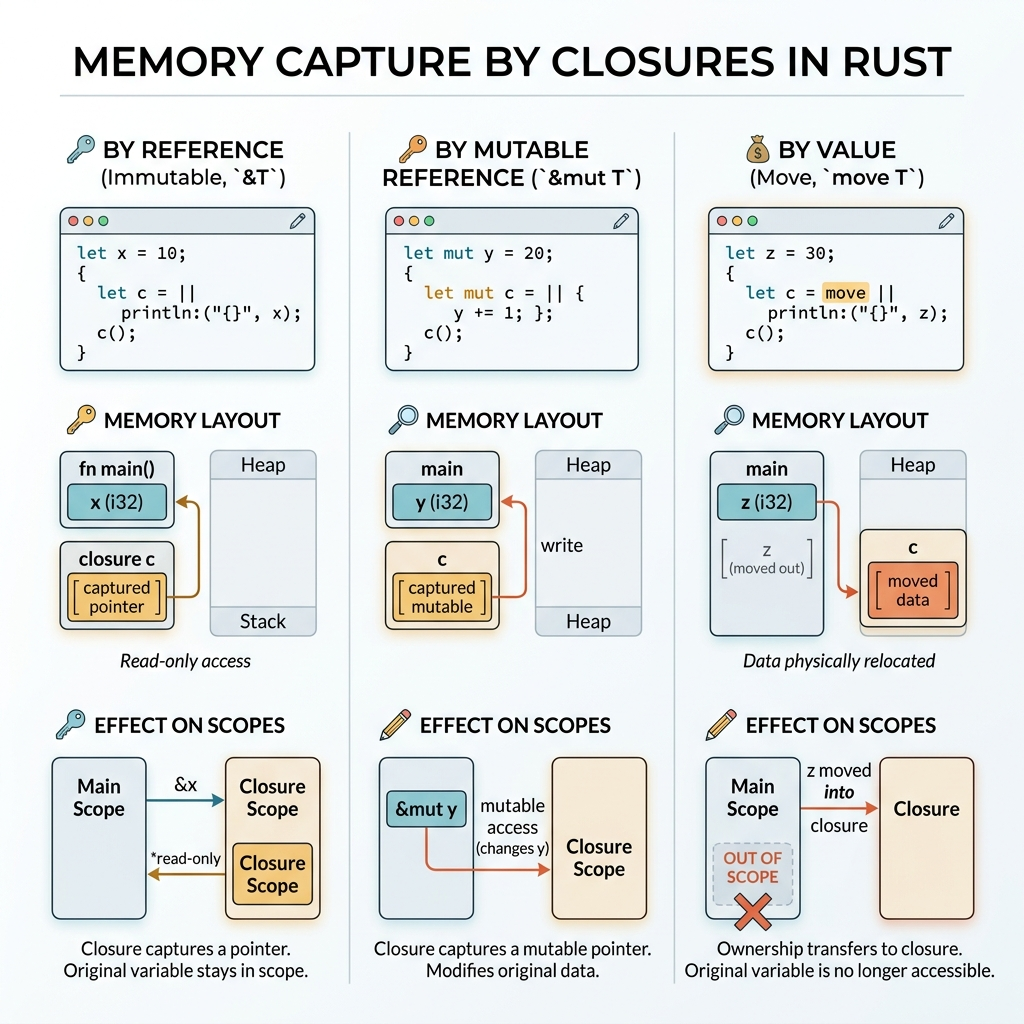
\includegraphics[width=\textwidth]{images/closure_memory.png}
    \caption{Memory layout showing how closures capture their environment via references versus taking ownership via the \texttt{move} keyword.}
\end{figure}

\begin{warningbox}
\textbf{Lifetimes and Captures:} When a closure captures by reference (immutable or mutable), the closure's lifetime is strictly bound by the shortest lifetime of the borrowed variables. If the closure attempts to outlive the variables it references, the compiler will raise a lifetime error to prevent dangling pointers.
\end{warningbox}

\section{The Closure Traits: \texttt{Fn}, \texttt{FnMut}, and \texttt{FnOnce}}
Because closures are essentially unique, anonymous structs generated on the fly, they cannot share a single concrete type known to the developer. Instead, they interact with the rest of the type system via traits. There are three functional traits in Rust, forming a strict hierarchy.

\subsection{\texttt{FnOnce}}
\texttt{FnOnce} is the foundational and most general closure trait. It indicates a closure that can be called \textit{at least once}. If a closure moves a captured variable out of its internal state (for example, dropping it or returning it), it fundamentally consumes its environment. Consequently, it can strictly only be executed exactly once. 

\begin{lstlisting}[language=Rust]
let range = vec![1, 2, 3];
// This closure consumes `range`, so it implements `FnOnce` 
// but it does not implement `FnMut` or `Fn`.
let consume = || {
    let _moved_range = range; 
};
consume();
// consume(); // ERROR: closure cannot be invoked more than once
\end{lstlisting}

\subsection{\texttt{FnMut}}
\texttt{FnMut} is a subtrait of \texttt{FnOnce}. It represents closures that can be called multiple times and have the ability to \textit{mutate} their captured environment. Because they modify state, invoking them requires a mutable reference to the closure itself. This trait is essential for closures that maintain an internal state, effectively "remembering" their past executions.

\begin{lstlisting}[language=Rust]
let mut sum = 0;
// Captures `sum` by mutable reference
let mut accumulate = |x| {
    sum += x;
    sum
};
println!("{}", accumulate(5)); // Prints 5
println!("{}", accumulate(7)); // Prints 12
\end{lstlisting}

\subsection{\texttt{Fn}}
\texttt{Fn} is a subtrait of \texttt{FnMut}. It represents closures that can be called multiple times without mutating their environment. They either capture no environment at all, or they strictly capture variables by immutable reference. Invoking an \texttt{Fn} closure does not require exclusive access, meaning it can be called repeatedly or even concurrently, behaving deterministically with fixed inputs.

\begin{notebox}
\textbf{Trait Hierarchy Context:} 
Every \texttt{Fn} is automatically an \texttt{FnMut}, and every \texttt{FnMut} is also an \texttt{FnOnce}. When writing a function that accepts a closure, you should request the most general trait possible to give the caller maximum flexibility: use \texttt{FnOnce} if you only call it once, \texttt{FnMut} if you must call it repeatedly in a loop, and \texttt{Fn} if you need to call it concurrently or require a lack of side-effects.
\end{notebox}

\section{Passing Closures as Arguments}
When designing APIs that accept closures, you must decide how to handle the anonymous types. There are two primary architectural approaches: Static Dispatch and Dynamic Dispatch.

\subsection{Static Dispatch (Monomorphization)}
The most common approach utilizes generic programming. You define a generic type parameter constrained by one of the closure traits.

\begin{lstlisting}[language=Rust]
fn apply<F>(value: i32, f: F) -> i32 
where 
    F: Fn(i32) -> i32 
{
    f(value)
}

let result = apply(5, |x| x * 2);
\end{lstlisting}

\textbf{Trade-offs:} This guarantees zero-cost abstraction. The compiler generates a distinct, specialized copy of the \texttt{apply} function for every specific closure type passed to it (monomorphization). Execution is extremely fast and allows full inlining, though it can slightly increase the final binary size.

\subsection{Dynamic Dispatch (Trait Objects)}
Alternatively, you can achieve dynamic polymorphism by passing the closure as a Trait Object, typically stored inside a \texttt{Box}.

\begin{lstlisting}[language=Rust]
struct PipelineStep {
    op: Box<dyn Fn(i32) -> i32>,
}

impl PipelineStep {
    fn execute(&self, x: i32) -> i32 {
        (self.op)(x)
    }
}
\end{lstlisting}

\begin{notebox}
\textbf{Dynamic Dispatch Mechanics:} A \texttt{Box<dyn Fn(i32) -> i32>} consists of a ``fat pointer'': one pointer directed to the closure's captured data (the anonymous struct) and another to a Virtual Method Table (VTable) containing the physical memory address of the function to execute.
\end{notebox}

\textbf{Trade-offs:} This prevents code bloat and uniquely allows you to store heterogeneous closures in the same collection (e.g., a \texttt{Vec<Box<dyn Fn(i32) -> i32>>}). However, it introduces a small runtime cost due to pointer indirection. Resolving the actual function call through the VTable requires an extra memory jump, which can slightly degrade CPU cache locality. It also acts as an optimization barrier, hindering the compiler from inlining the closure body.

\section{Returning Closures}
Returning a closure from a function introduces complexity. Since closures are anonymous types generated by the compiler, you cannot explicitly name the return type. Instead, Rust provides the \texttt{impl Trait} syntax to describe the output generically.

Crucially, a closure returned from a function \textit{must} outlive the function call itself. If the closure captures local variables by reference, those references would become dangling the moment the function returns and its stack frame is destroyed. Therefore, returning a closure almost always requires the \texttt{move} keyword to force ownership of the captured variables, making the closure entirely self-sufficient.

\begin{lstlisting}[language=Rust]
fn make_multiplier(factor: i32) -> impl Fn(i32) -> i32 {
    // `move` forces the closure to take ownership of `factor`.
    // Without `move`, `factor` would be dropped at the end of the function,
    // leaving a dangling reference inside the closure.
    move |x| x * factor
}

let double = make_multiplier(2);
println!("{}", double(10)); // Prints 20
\end{lstlisting}

\subsection{Stateful Closures: The Generator Pattern}
Combining \texttt{move} and \texttt{impl FnMut} empowers us to create powerful stateful objects, such as generators that remember their past executions and maintain state across invocations.

\begin{lstlisting}[language=Rust]
fn make_identifier_generator(prefix: String) -> impl FnMut() -> String {
    let mut count = 0;
    
    move || {
        count += 1;
        format!("{}{}", prefix, count)
    }
}

let mut gen = make_identifier_generator(String::from("id_"));
println!("{}", gen()); // Output: id_1
println!("{}", gen()); // Output: id_2
\end{lstlisting}

In this pattern, the closure carries its own encapsulated state (\texttt{count} and \texttt{prefix}). Each invocation safely updates the internal counter and produces a fresh identifier. The state is strictly bound to the lifetime of the returned closure instance.

\section*{End-of-Chapter Exam Questions}

\begin{exambox}
\textbf{Question 1: Conceptual Understanding} \\
Explain the hierarchical relationship between the \texttt{Fn}, \texttt{FnMut}, and \texttt{FnOnce} traits. If a function signature requires a parameter of type \texttt{F: FnOnce()}, can you pass a closure that implements \texttt{Fn} to it? Why or why not?

\vspace{1em}
\textbf{Question 2: Memory \& Ownership} \\
Examine the following code snippet:
\begin{lstlisting}[language=Rust]
fn create_greeter(name: String) -> impl Fn() -> String {
    || format!("Hello, {}!", name)
}
\end{lstlisting}
This code will fail to compile. Explain the exact reason for the compilation error in terms of memory management and lifetimes. Then, rewrite the function to correctly resolve the issue.

\vspace{1em}
\textbf{Question 3: Architecture \& Dispatch} \\
You are designing a GUI framework in Rust where a \texttt{Button} struct needs to dynamically store a collection of \texttt{onClick} callbacks. The callbacks might be entirely different closures that take no arguments. Should you use generic parameters (static dispatch) or trait objects (dynamic dispatch) for the \texttt{Button}'s structure to support multiple, varying listeners in a vector? Discuss the trade-offs of your choice.
\end{exambox}
